\chapter{Comparison of Experimental and Monte Carlo Distributions} \label{app:distributions}
This appendix compares the distributions of reconstructued quantities measured in experiment
to those generated by \textit{SIMC}.
Error bars are statistical only and the distributions are normalized to each other.
\begin{figure}[!h]
    \centering
    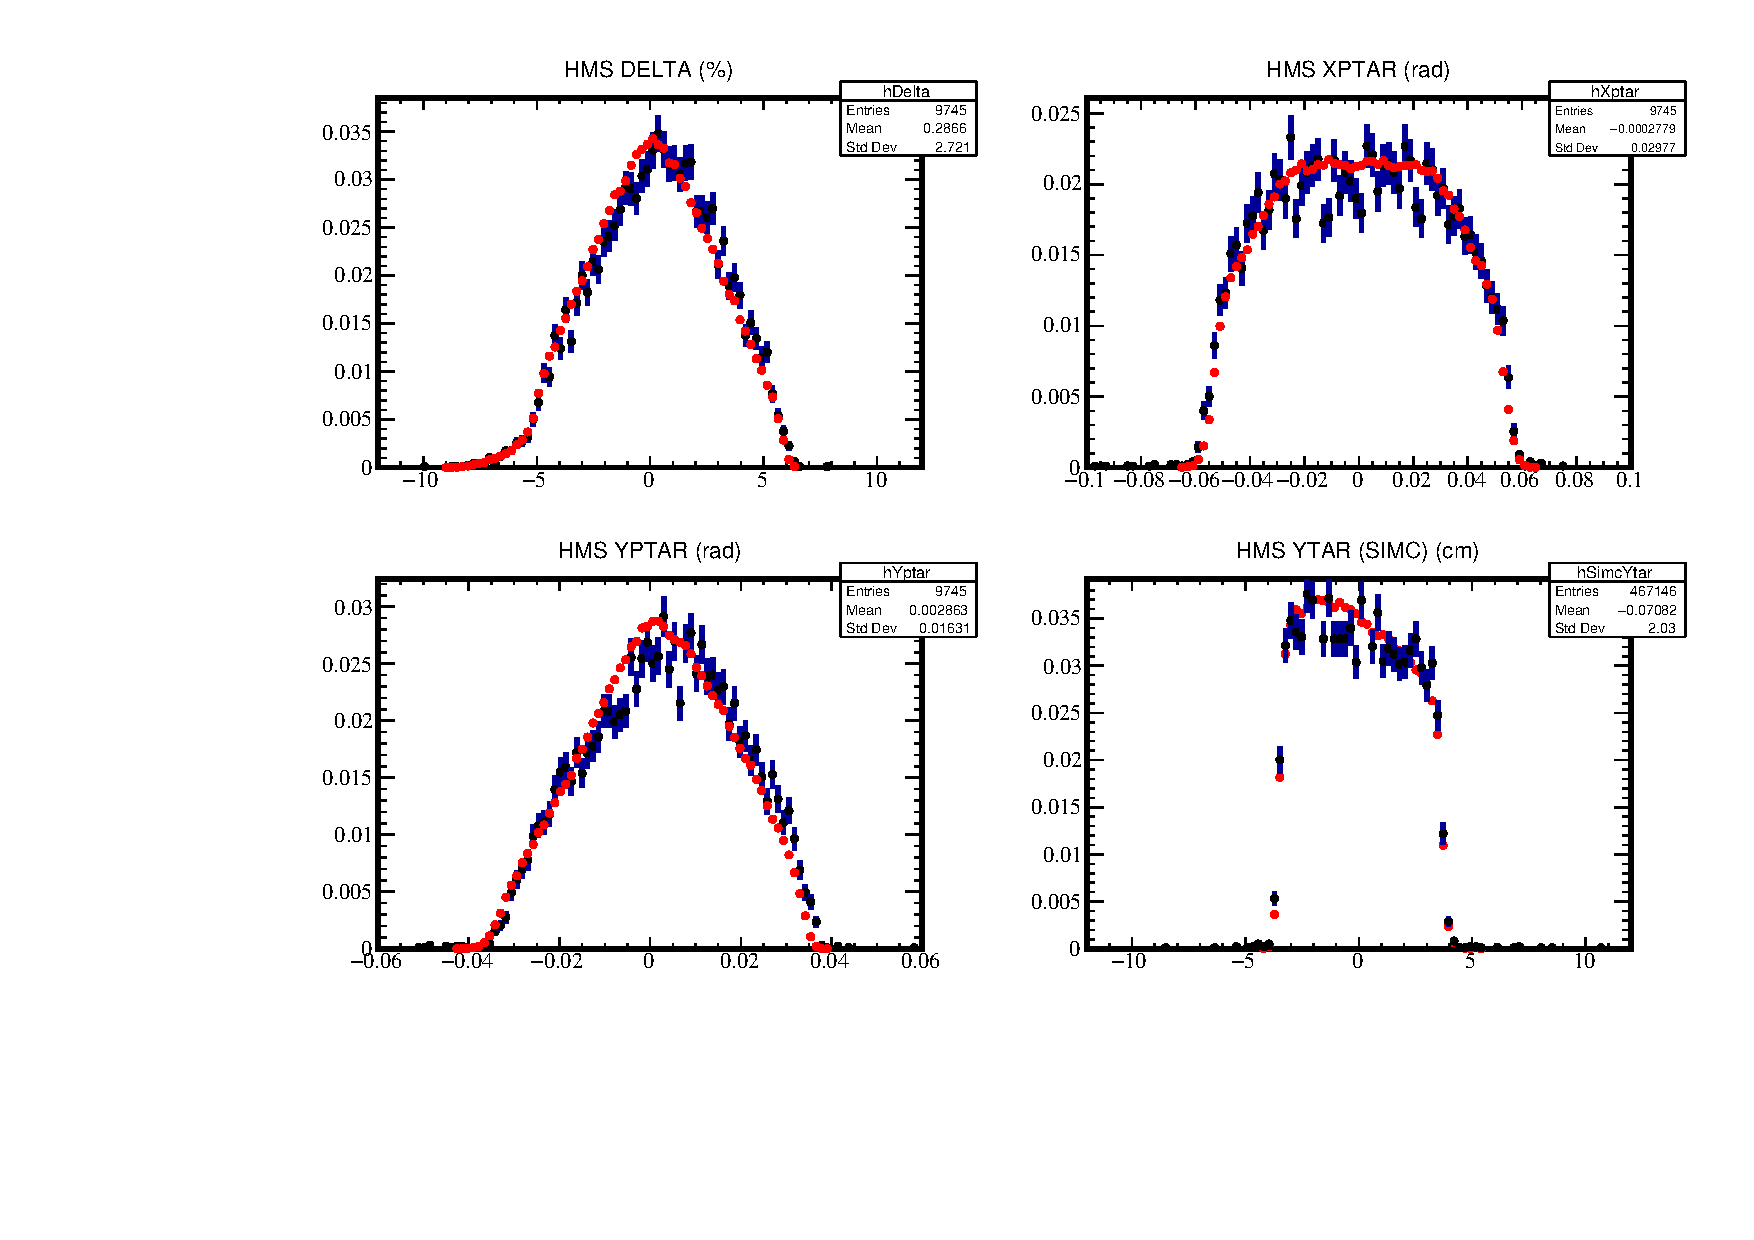
\includegraphics[page=1,width=1.0\textwidth]{pass5_report/Report_h8.pdf}
    \caption{
            Experimental (in blue) and Monte Carlo (in red) distributions of
            target quantities reconstructed from the HMS for
            the $LH_2$ target at $Q^2=\SI{8.0}{\giga\electronvolt\squared}$.
            }
    \label{fig:Report_h8.pdf}
\end{figure}


\begin{figure}[!h]
    \centering
    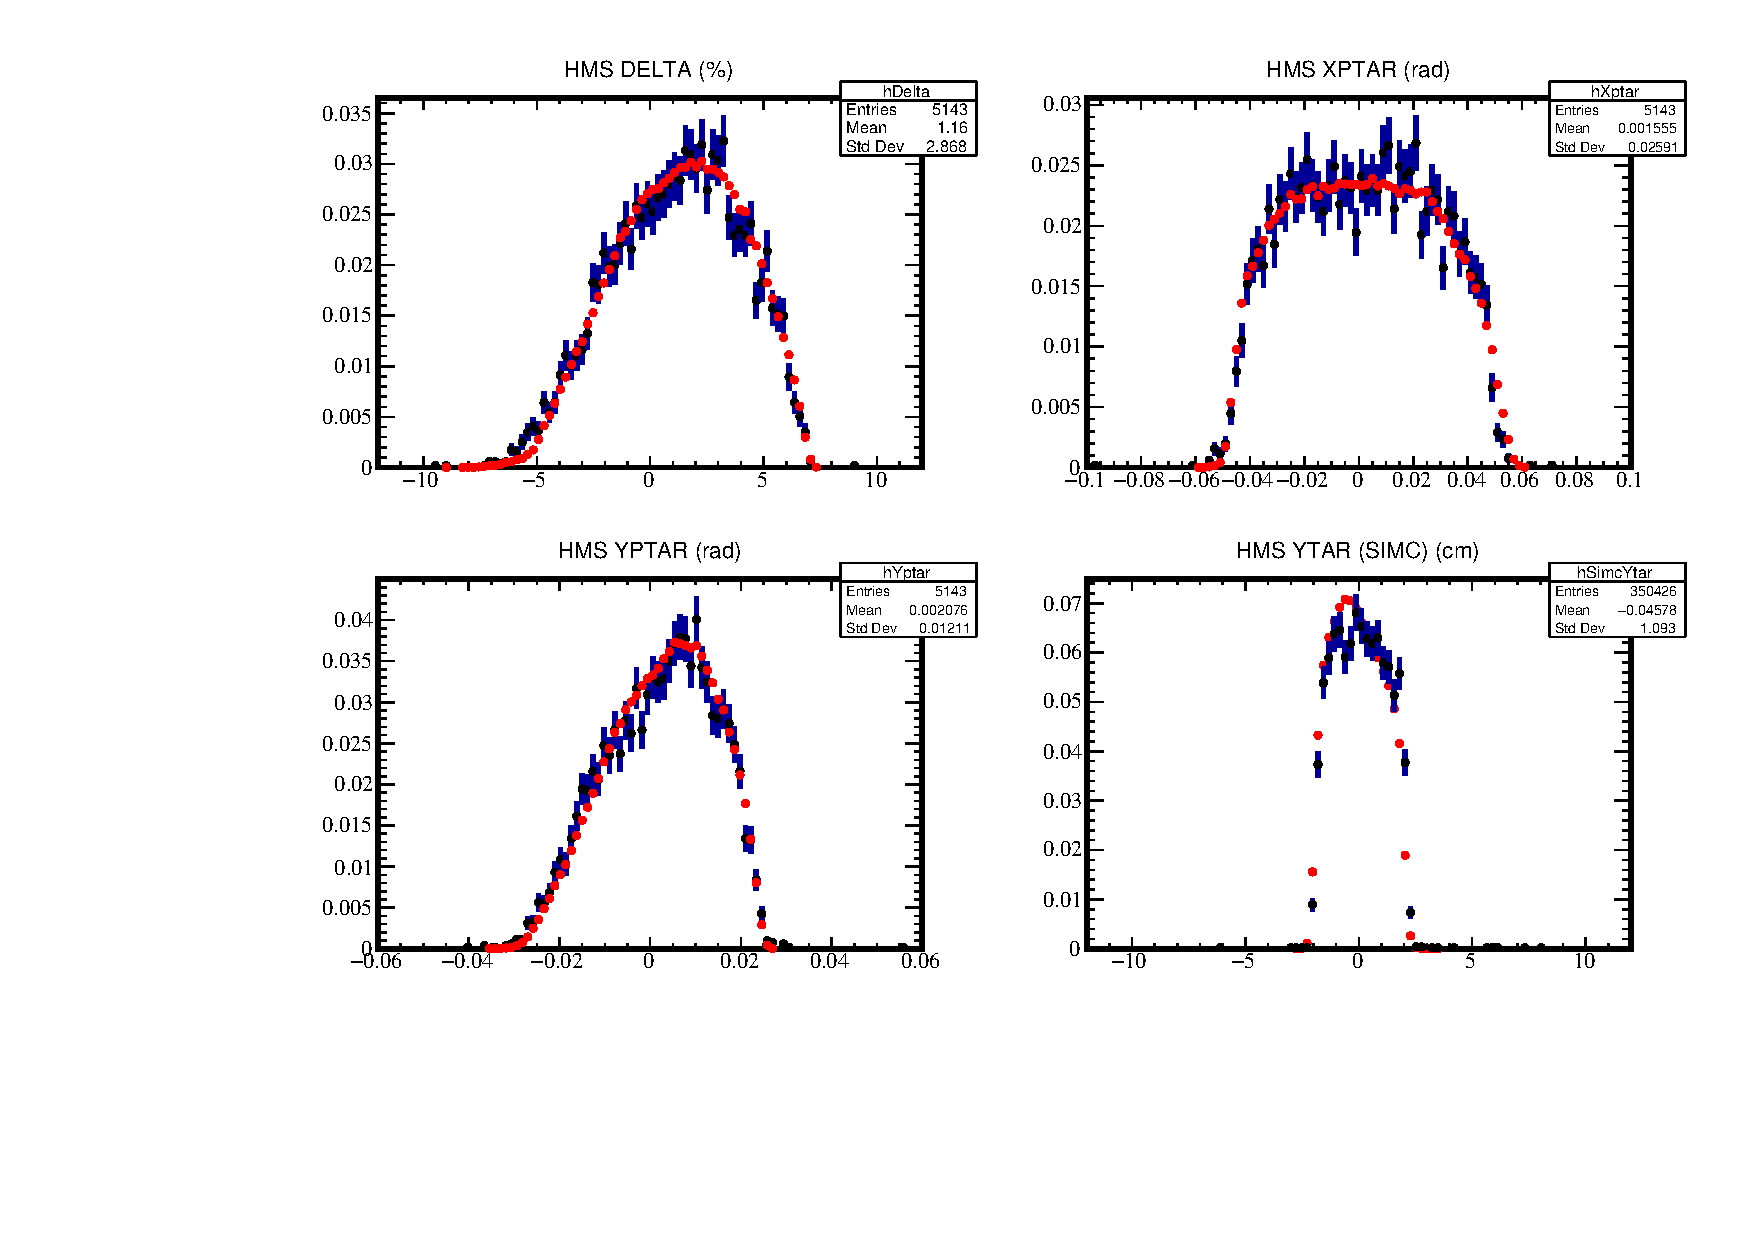
\includegraphics[page=1,width=1.0\textwidth]{pass5_report/Report_h95sm.pdf}
    \caption{
            Experimental (in blue) and Monte Carlo (in red) distributions of
            target quantities reconstructed from the HMS for
            the $LH_2$ target at $Q^2=\SI{9.5}{\giga\electronvolt\squared}$.
            }
    \label{fig:Report_h95sm.pdf}
\end{figure}


\begin{figure}[!h]
    \centering
    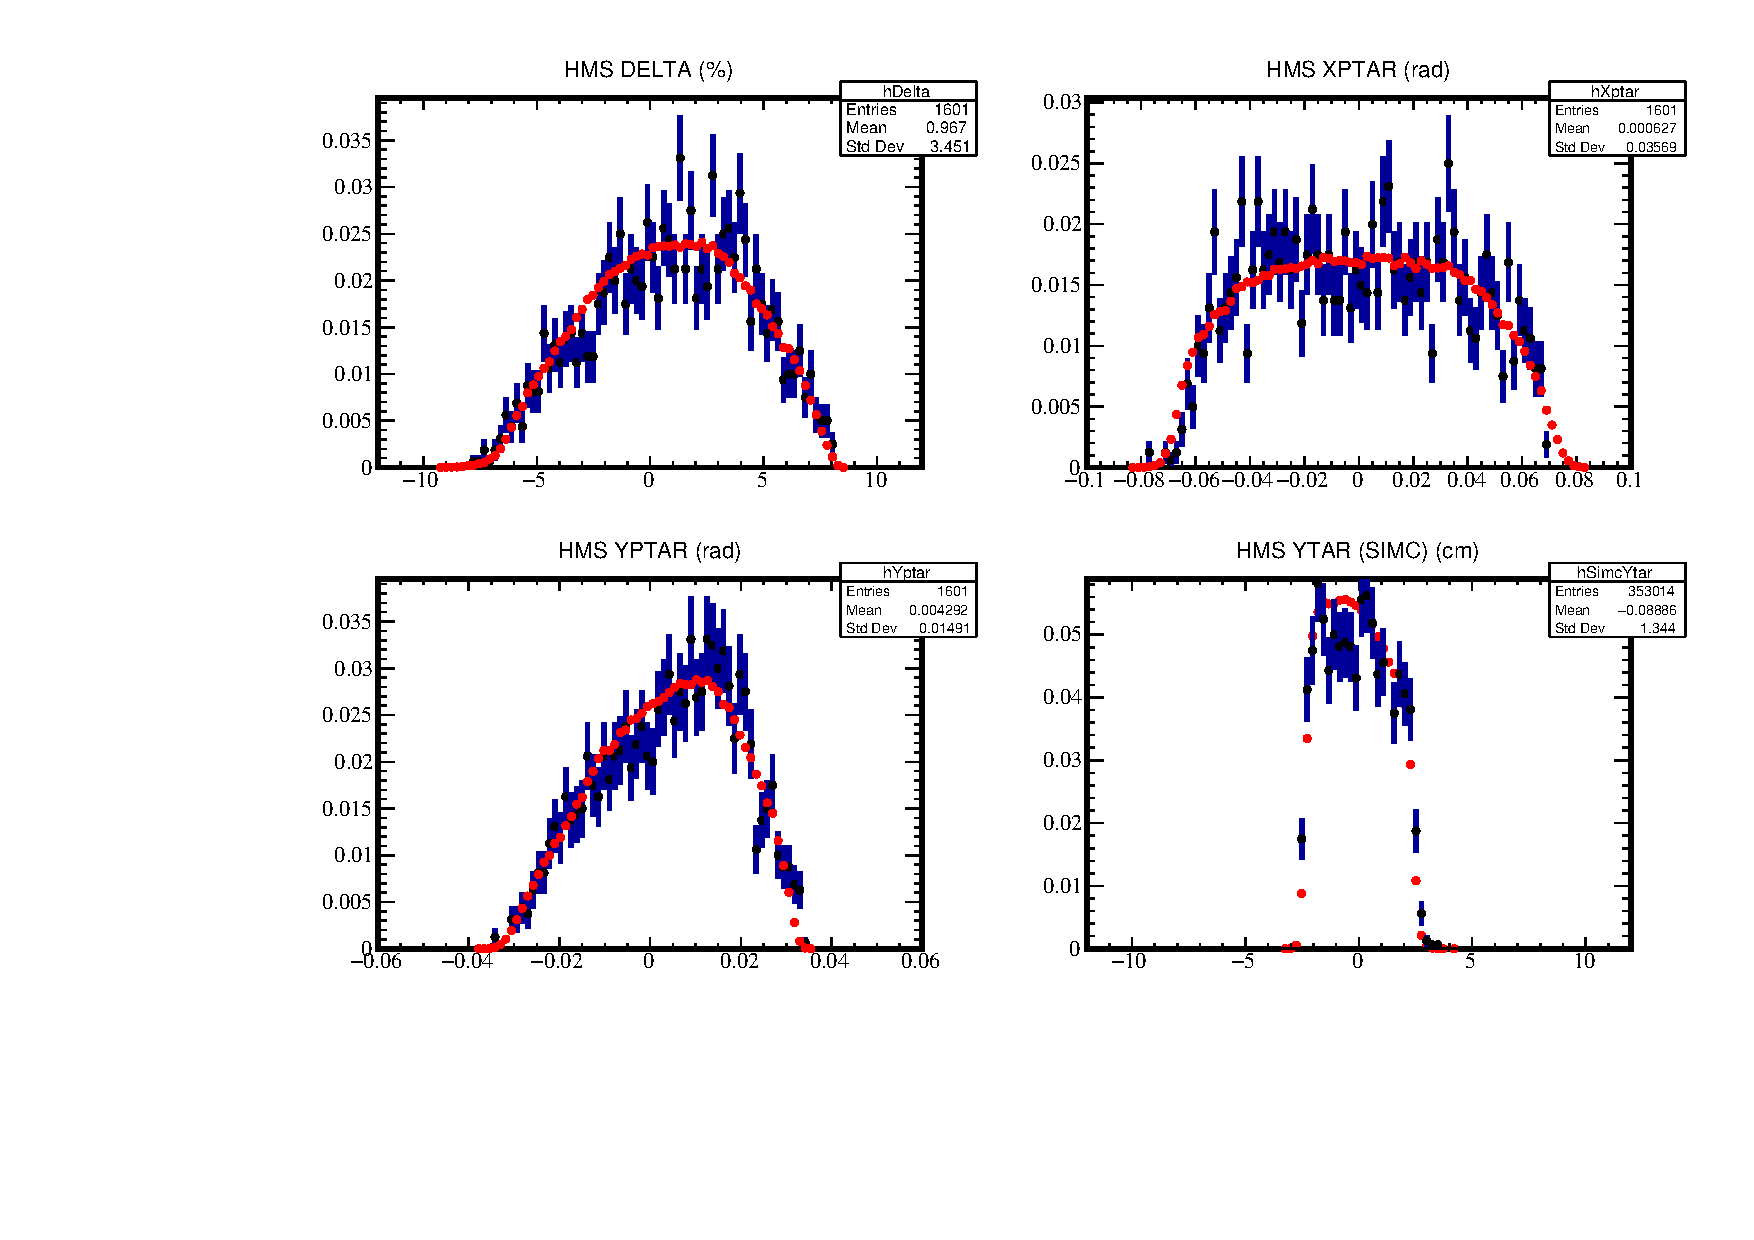
\includegraphics[page=1,width=1.0\textwidth]{pass5_report/Report_h115.pdf}
    \caption{
            Experimental (in blue) and Monte Carlo (in red) distributions of
            target quantities reconstructed from the HMS for
            the $LH_2$ target at $Q^2=\SI{11.5}{\giga\electronvolt\squared}$.
            }
    \label{fig:Report_h115.pdf}
\end{figure}


\begin{figure}[!h]
    \centering
    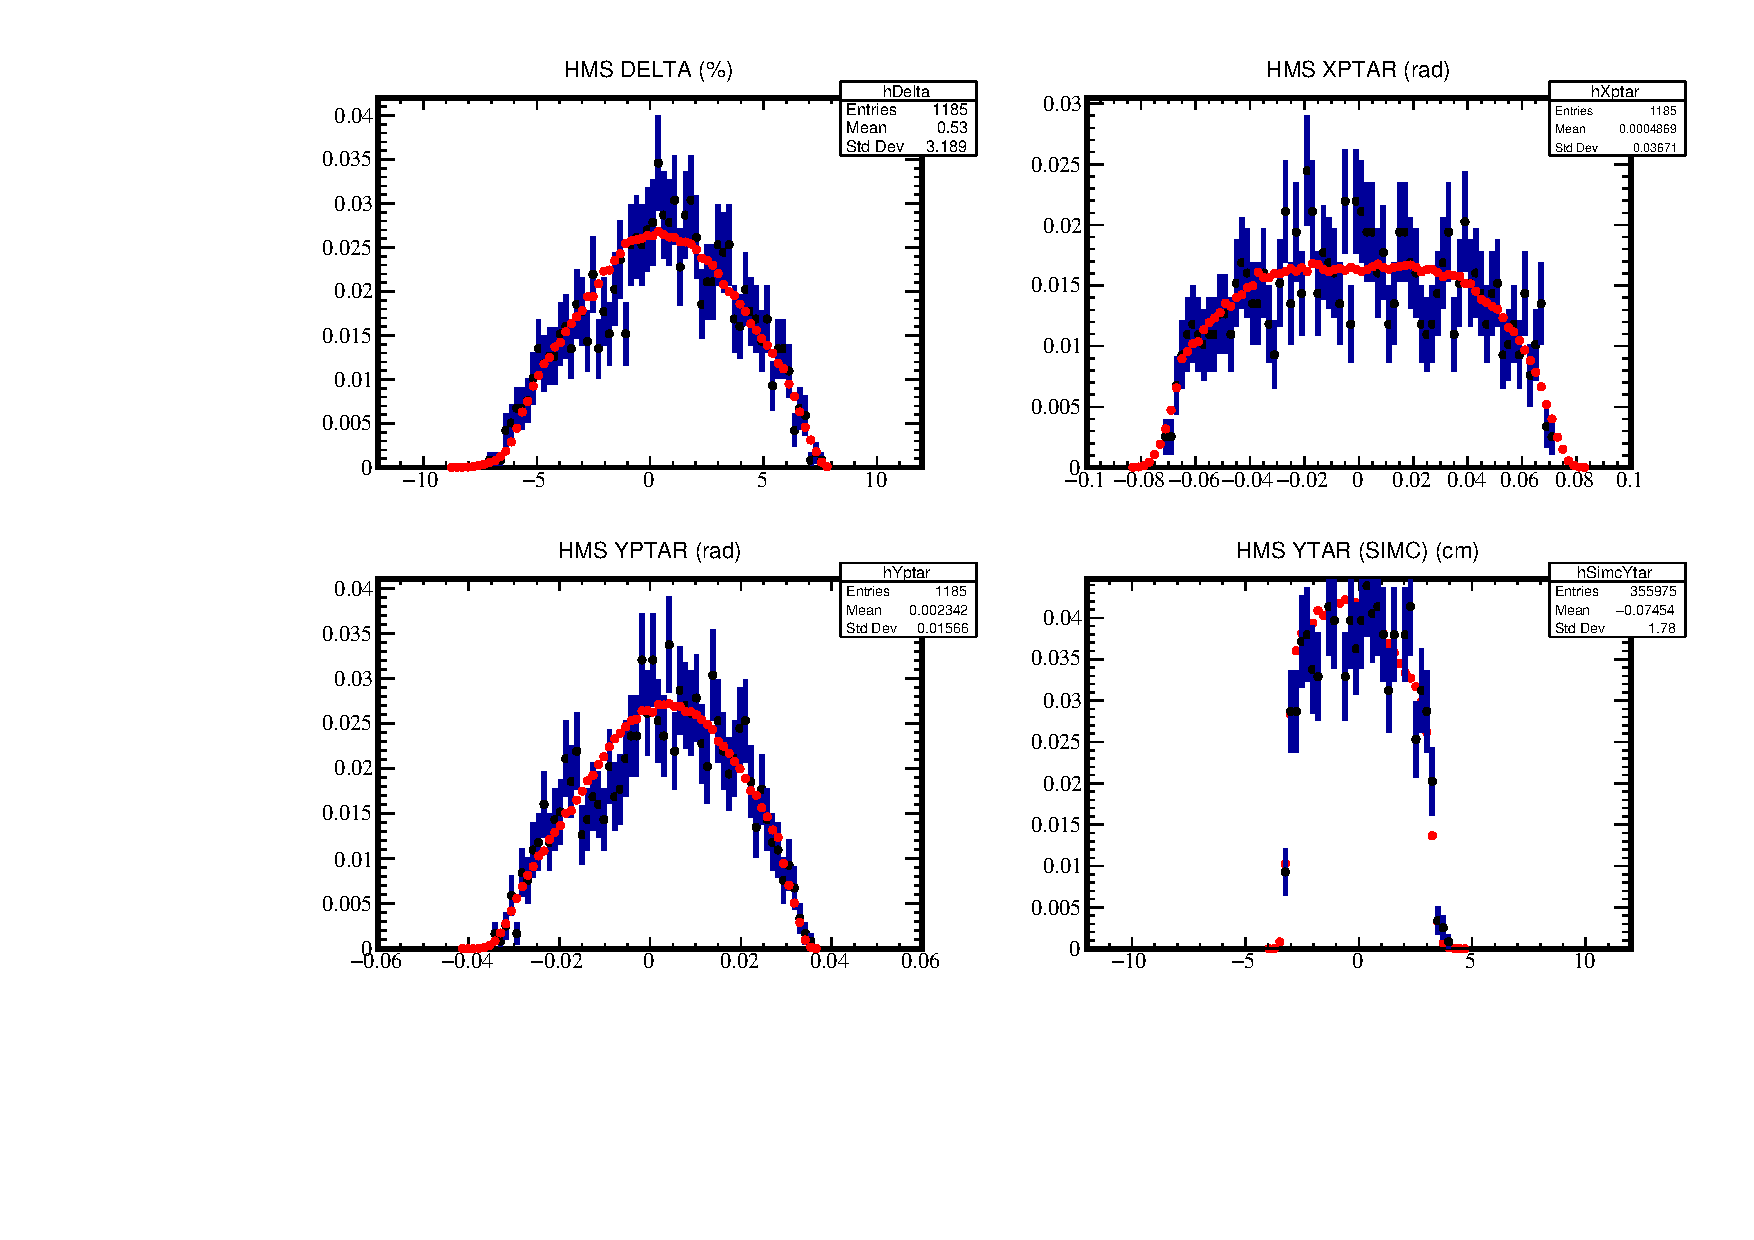
\includegraphics[page=1,width=1.0\textwidth]{pass5_report/Report_h143.pdf}
    \caption{
            Experimental (in blue) and Monte Carlo (in red) distributions of
            target quantities reconstructed from the HMS for
            the $LH_2$ target at $Q^2=\SI{14.2}{\giga\electronvolt\squared}$.
            }
    \label{fig:Report_h143.pdf}
\end{figure}


\begin{figure}[!h]
    \centering
    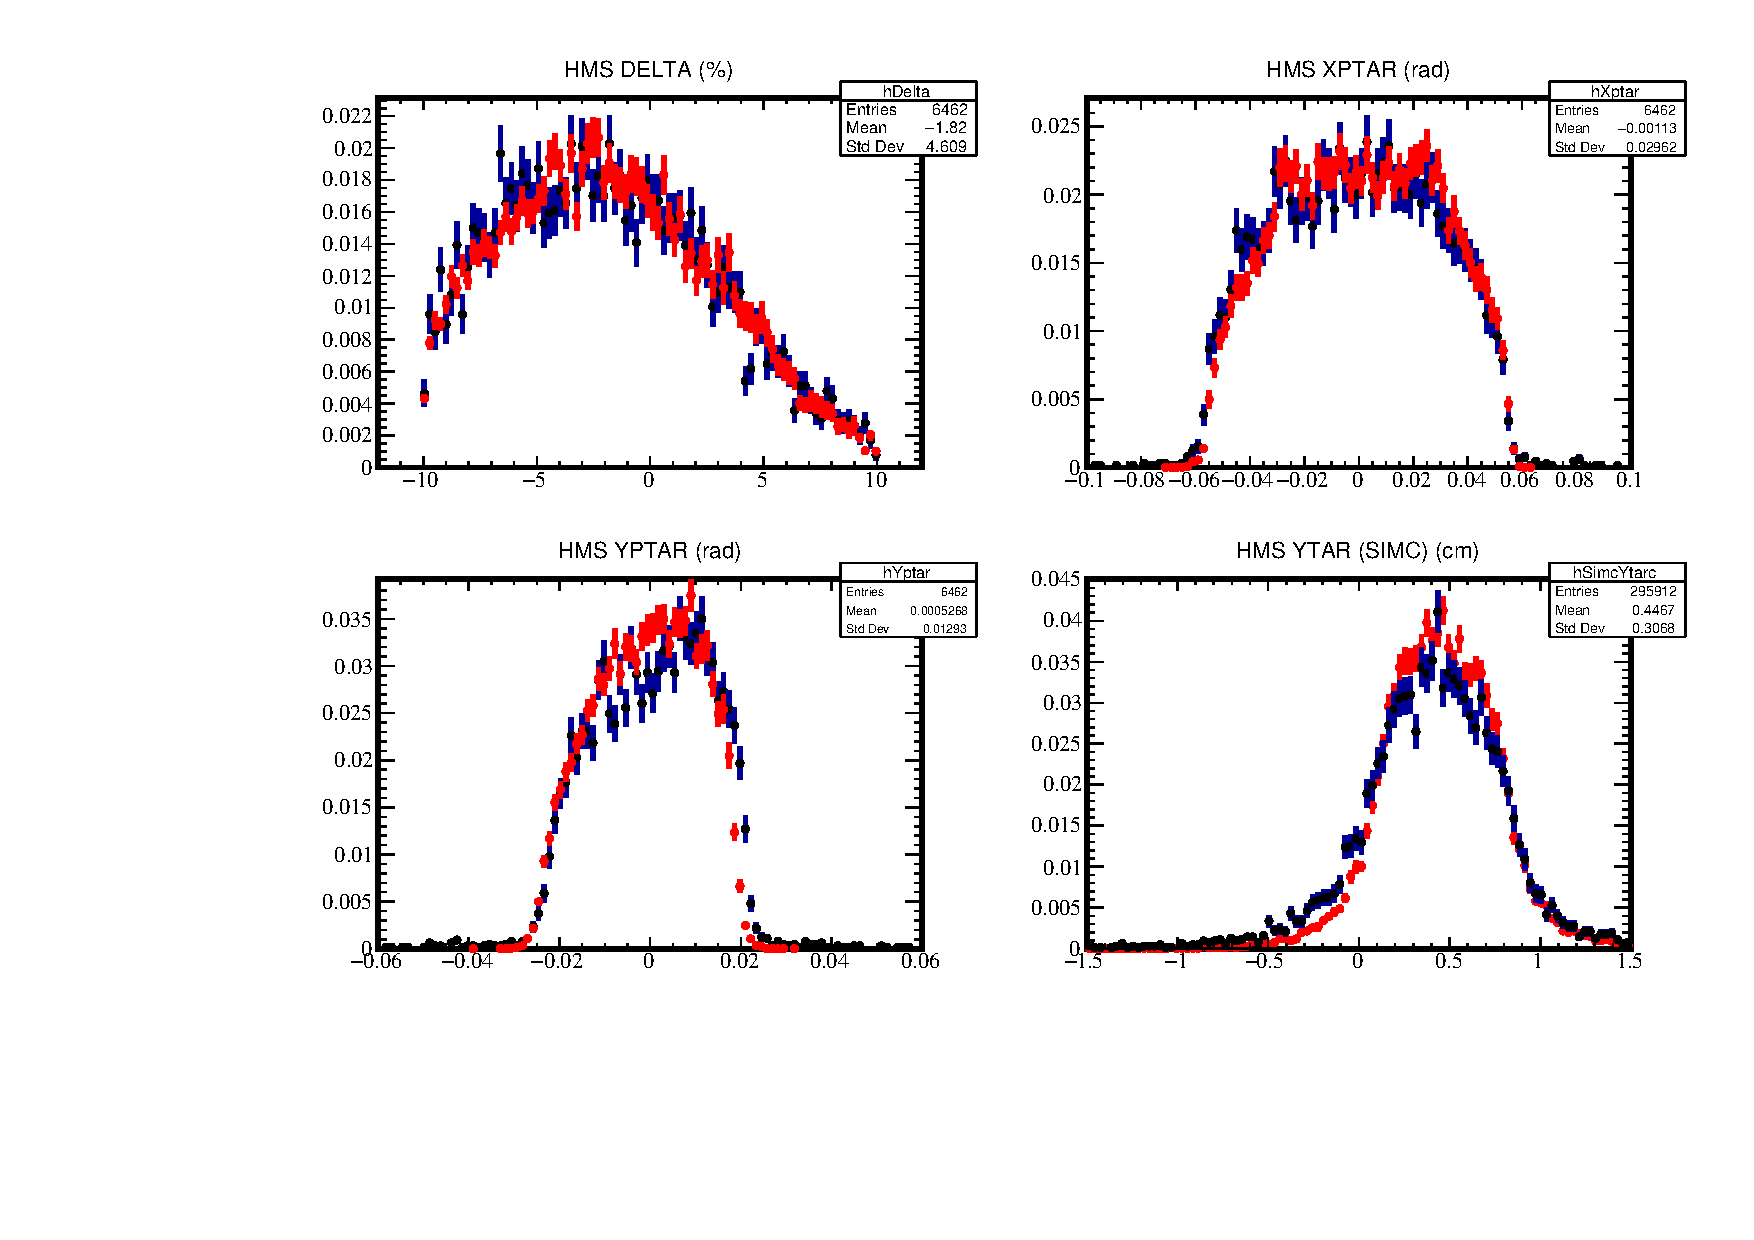
\includegraphics[page=1,width=1.0\textwidth]{pass5_report/Report_c12_8.pdf}
    \caption{
            Experimental (in blue) and Monte Carlo (in red) distributions of
            target quantities reconstructed from the HMS for
            the ${}^{12}C$ target at $Q^2=\SI{8.0}{\giga\electronvolt\squared}$.
            }
    \label{fig:Report_c12_8.pdf}
\end{figure}


\begin{figure}[!h]
    \centering
    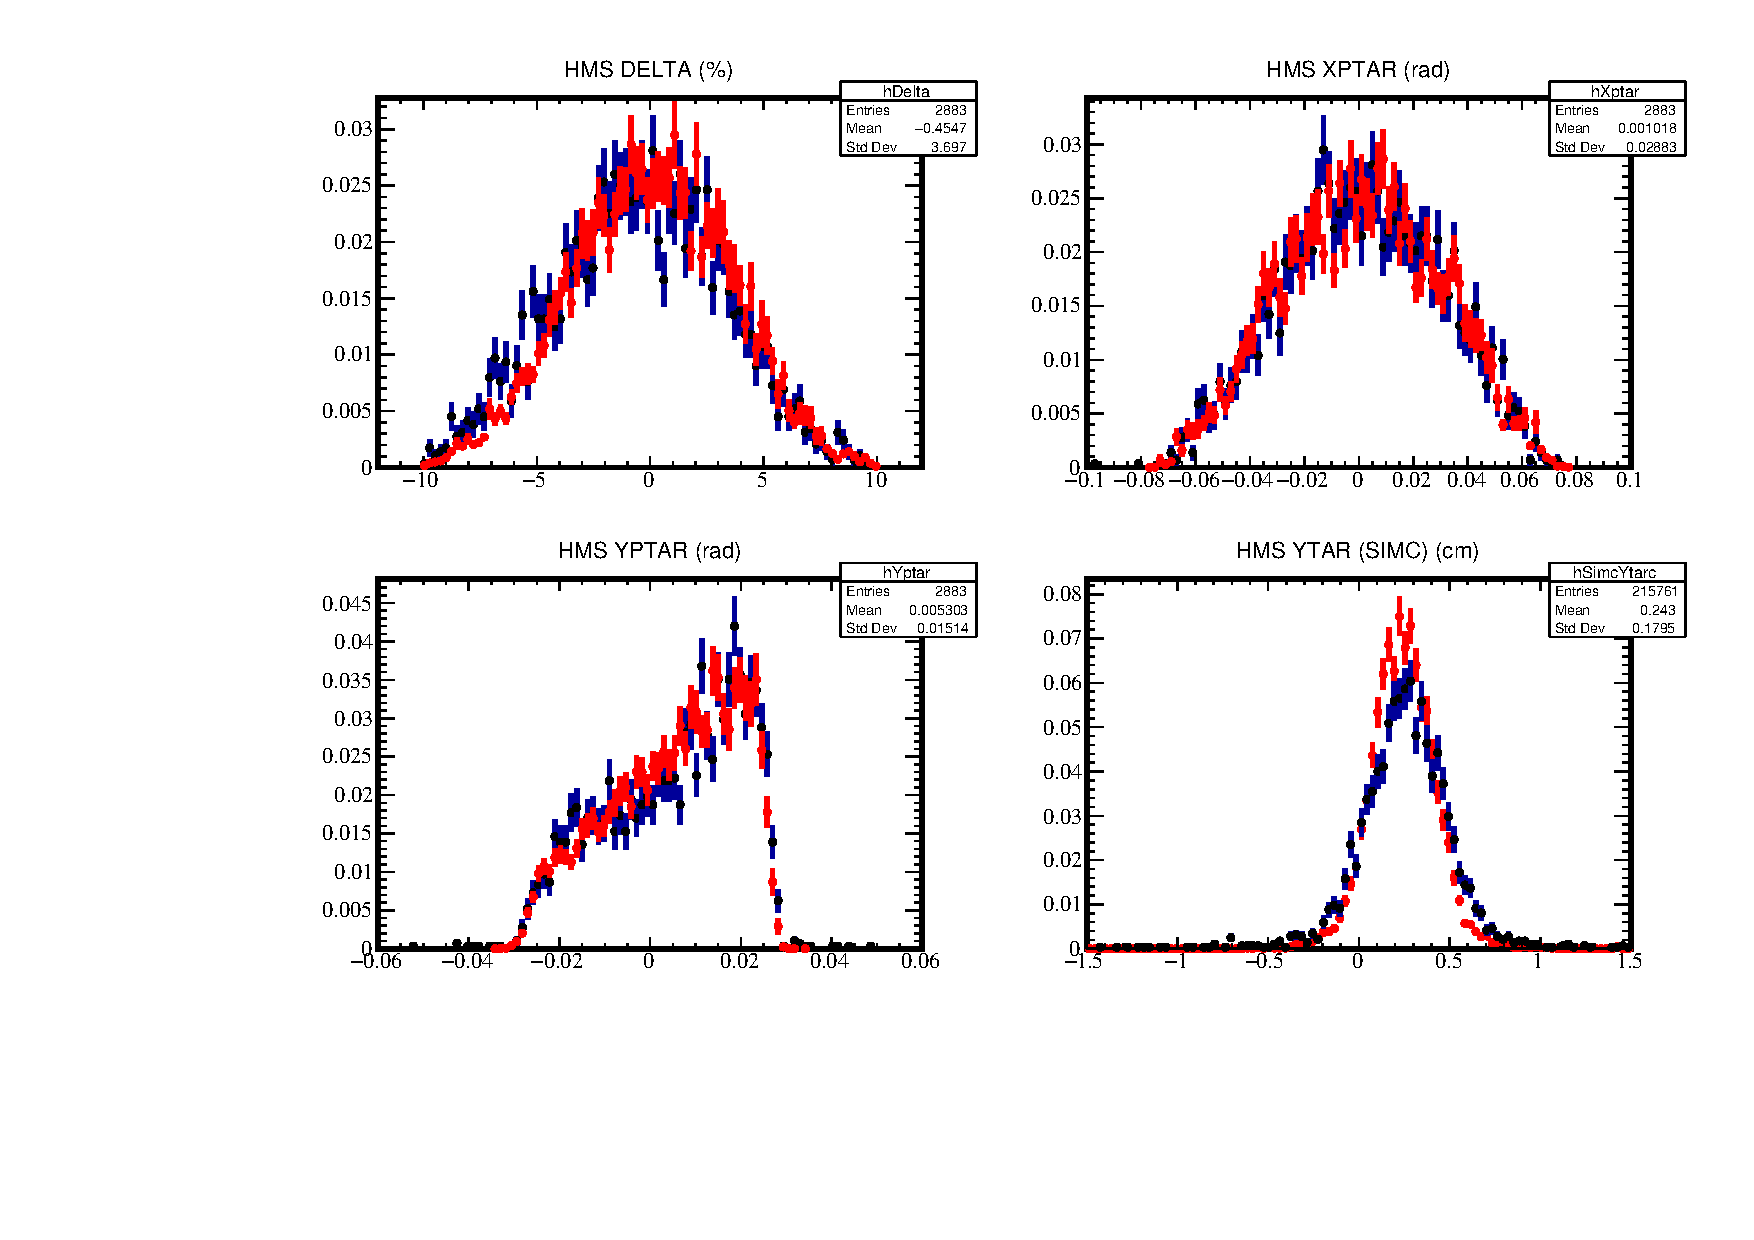
\includegraphics[page=1,width=1.0\textwidth]{pass5_report/Report_c95.pdf}
    \caption{
            Experimental (in blue) and Monte Carlo (in red) distributions of
            target quantities reconstructed from the HMS for
            the ${}^{12}C$ target at $Q^2=\SI{9.5}{\giga\electronvolt\squared}$.
            }
    \label{fig:Report_c95.pdf}
\end{figure}


\begin{figure}[!h]
    \centering
    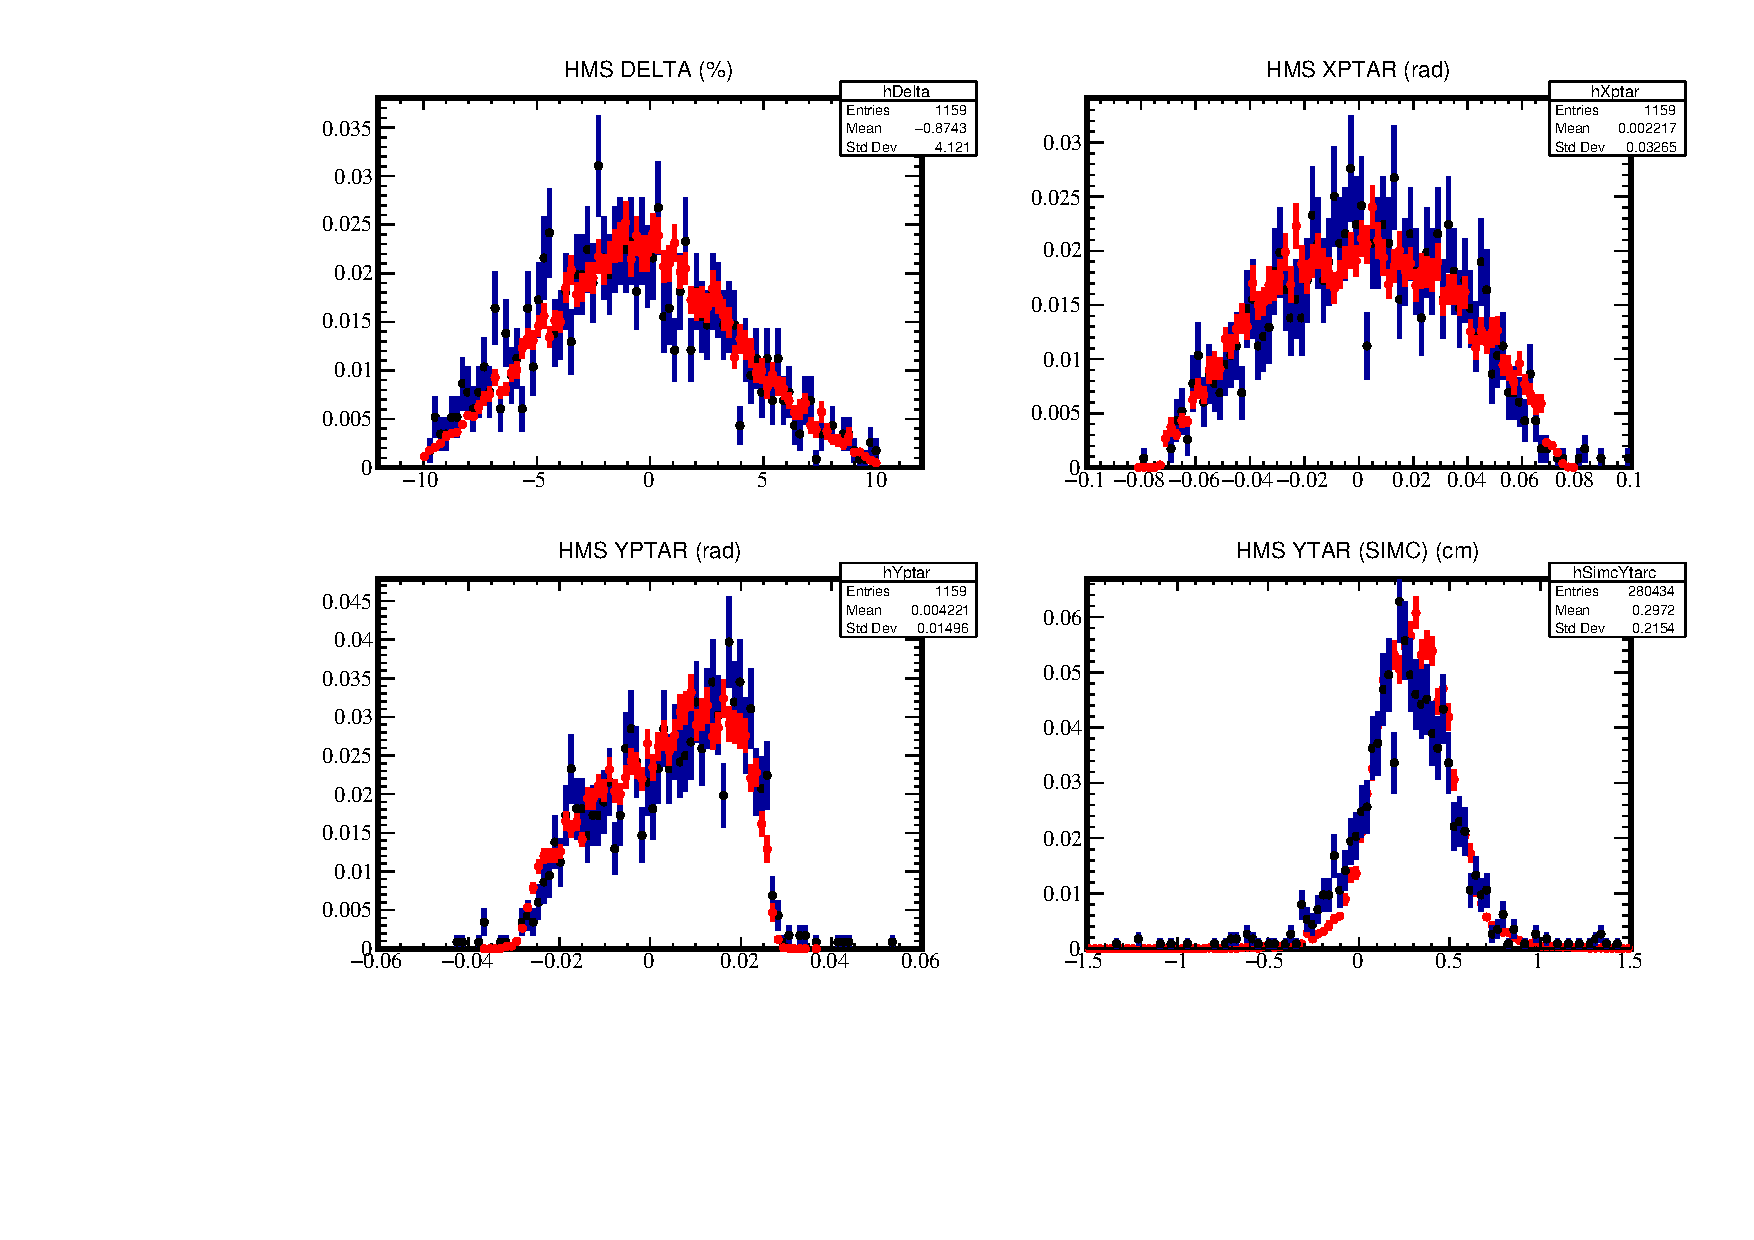
\includegraphics[page=1,width=1.0\textwidth]{pass5_report/Report_c115.pdf}
    \caption{
            Experimental (in blue) and Monte Carlo (in red) distributions of
            target quantities reconstructed from the HMS for
            the ${}^{12}C$ target at $Q^2=\SI{11.5}{\giga\electronvolt\squared}$.
            }
    \label{fig:Report_c115.pdf}
\end{figure}


\begin{figure}[!h]
    \centering
    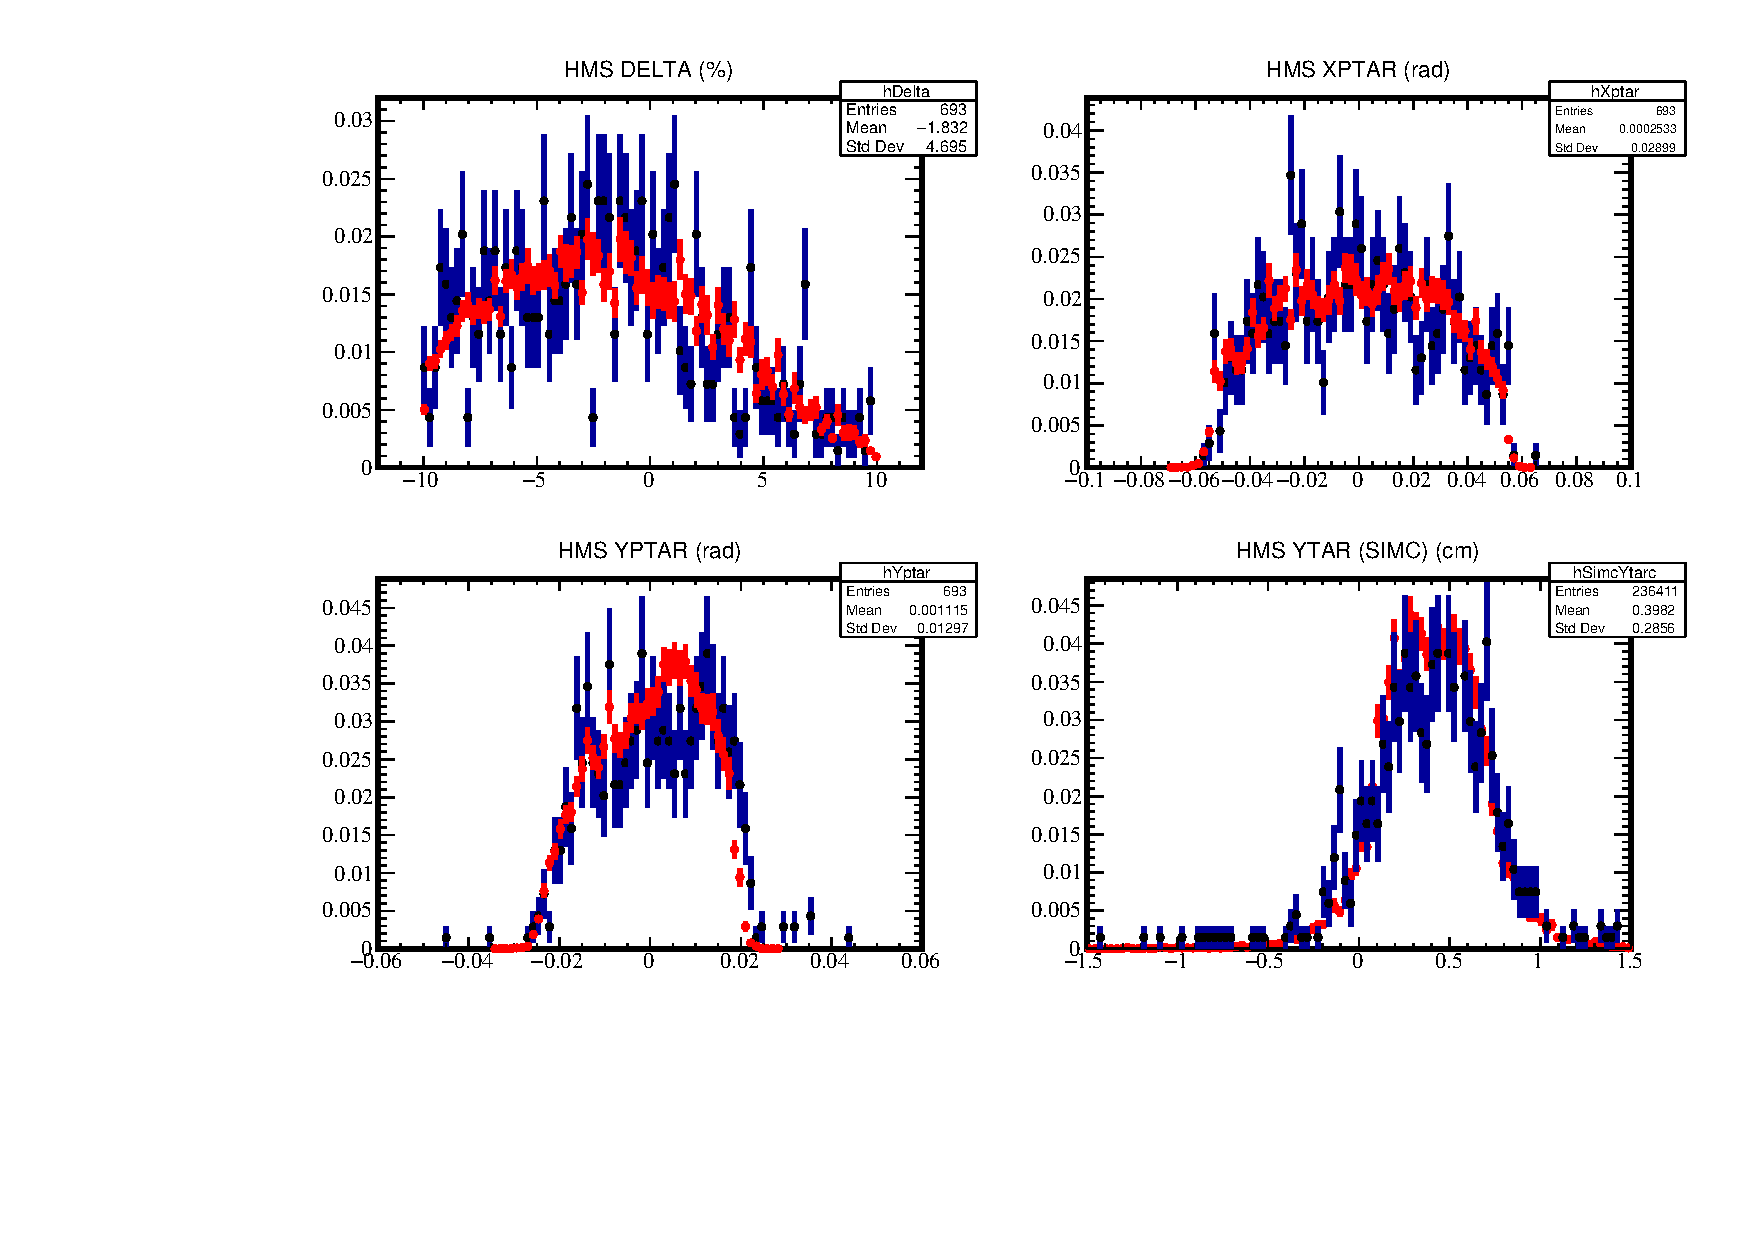
\includegraphics[page=1,width=1.0\textwidth]{pass5_report/Report_c143_sm.pdf}
    \caption{
            Experimental (in blue) and Monte Carlo (in red) distributions of
            target quantities reconstructed from the HMS for
            the ${}^{12}C$ target at $Q^2=\SI{14.2}{\giga\electronvolt\squared}$.
            }
    \label{fig:Report_c143_sm.pdf}
\end{figure}


\begin{figure}[!h]
    \centering
    \includegraphics[page=2,width=1.0\textwidth]{pass5_report/Report_h8.pdf}
    \caption{
            Experimental (in blue) and Monte Carlo (in red) distributions of
            target quantities reconstructed from the SHMS for
            the $LH_2$ target at $Q^2=\SI{8.0}{\giga\electronvolt\squared}$.
            }
    \label{fig:Report_h8.pdf}
\end{figure}


\begin{figure}[!h]
    \centering
    \includegraphics[page=2,width=1.0\textwidth]{pass5_report/Report_h95sm.pdf}
    \caption{
            Experimental (in blue) and Monte Carlo (in red) distributions of
            target quantities reconstructed from the SHMS for
            the $LH_2$ target at $Q^2=\SI{9.5}{\giga\electronvolt\squared}$.
            }
    \label{fig:Report_h95sm.pdf}
\end{figure}


\begin{figure}[!h]
    \centering
    \includegraphics[page=2,width=1.0\textwidth]{pass5_report/Report_h115.pdf}
    \caption{
            Experimental (in blue) and Monte Carlo (in red) distributions of
            target quantities reconstructed from the SHMS for
            the $LH_2$ target at $Q^2=\SI{11.5}{\giga\electronvolt\squared}$.
            }
    \label{fig:Report_h115.pdf}
\end{figure}


\begin{figure}[!h]
    \centering
    \includegraphics[page=2,width=1.0\textwidth]{pass5_report/Report_h143.pdf}
    \caption{
            Experimental (in blue) and Monte Carlo (in red) distributions of
            target quantities reconstructed from the SHMS for
            the $LH_2$ target at $Q^2=\SI{14.2}{\giga\electronvolt\squared}$.
            }
    \label{fig:Report_h143.pdf}
\end{figure}


\begin{figure}[!h]
    \centering
    \includegraphics[page=2,width=1.0\textwidth]{pass5_report/Report_c12_8.pdf}
    \caption{
            Experimental (in blue) and Monte Carlo (in red) distributions of
            target quantities reconstructed from the SHMS for
            the ${}^{12}C$ target at $Q^2=\SI{8.0}{\giga\electronvolt\squared}$.
            }
    \label{fig:Report_c12_8.pdf}
\end{figure}


\begin{figure}[!h]
    \centering
    \includegraphics[page=2,width=1.0\textwidth]{pass5_report/Report_c95.pdf}
    \caption{
            Experimental (in blue) and Monte Carlo (in red) distributions of
            target quantities reconstructed from the SHMS for
            the ${}^{12}C$ target at $Q^2=\SI{9.5}{\giga\electronvolt\squared}$.
            }
    \label{fig:Report_c95.pdf}
\end{figure}


\begin{figure}[!h]
    \centering
    \includegraphics[page=2,width=1.0\textwidth]{pass5_report/Report_c115.pdf}
    \caption{
            Experimental (in blue) and Monte Carlo (in red) distributions of
            target quantities reconstructed from the SHMS for
            the ${}^{12}C$ target at $Q^2=\SI{11.5}{\giga\electronvolt\squared}$.
            }
    \label{fig:Report_c115.pdf}
\end{figure}


\begin{figure}[!h]
    \centering
    \includegraphics[page=2,width=1.0\textwidth]{pass5_report/Report_c143_sm.pdf}
    \caption{
            Experimental (in blue) and Monte Carlo (in red) distributions of
            target quantities reconstructed from the SHMS for
            the ${}^{12}C$ target at $Q^2=\SI{14.2}{\giga\electronvolt\squared}$.
            }
    \label{fig:Report_c143_sm.pdf}
\end{figure}


\begin{figure}[!h]
    \centering
    \includegraphics[page=3,width=1.0\textwidth]{pass5_report/Report_h8.pdf}
    \caption{
            Experimental (in blue) and Monte Carlo (in red) distributions of
            reconstructed physics quantities for
            the $LH_2$ target at $Q^2=\SI{8.0}{\giga\electronvolt\squared}$.
            }
    \label{fig:Report_h8.pdf}
\end{figure}


\begin{figure}[!h]
    \centering
    \includegraphics[page=3,width=1.0\textwidth]{pass5_report/Report_h95sm.pdf}
    \caption{
            Experimental (in blue) and Monte Carlo (in red) distributions of
            reconstructed physics quantities for
            the $LH_2$ target at $Q^2=\SI{9.5}{\giga\electronvolt\squared}$.
            }
    \label{fig:Report_h95sm.pdf}
\end{figure}


\begin{figure}[!h]
    \centering
    \includegraphics[page=3,width=1.0\textwidth]{pass5_report/Report_h115.pdf}
    \caption{
            Experimental (in blue) and Monte Carlo (in red) distributions of
            reconstructed physics quantities for
            the $LH_2$ target at $Q^2=\SI{11.5}{\giga\electronvolt\squared}$.
            }
    \label{fig:Report_h115.pdf}
\end{figure}


\begin{figure}[!h]
    \centering
    \includegraphics[page=3,width=1.0\textwidth]{pass5_report/Report_h143.pdf}
    \caption{
            Experimental (in blue) and Monte Carlo (in red) distributions of
            reconstructed physics quantities for
            the $LH_2$ target at $Q^2=\SI{14.2}{\giga\electronvolt\squared}$.
            }
    \label{fig:Report_h143.pdf}
\end{figure}


\begin{figure}[!h]
    \centering
    \includegraphics[page=3,width=1.0\textwidth]{pass5_report/Report_c12_8.pdf}
    \caption{
            Experimental (in blue) and Monte Carlo (in red) distributions of
            reconstructed physics quantities for
            the ${}^{12}C$ target at $Q^2=\SI{8.0}{\giga\electronvolt\squared}$.
            }
    \label{fig:Report_c12_8.pdf}
\end{figure}


\begin{figure}[!h]
    \centering
    \includegraphics[page=3,width=1.0\textwidth]{pass5_report/Report_c95.pdf}
    \caption{
            Experimental (in blue) and Monte Carlo (in red) distributions of
            reconstructed physics quantities for
            the ${}^{12}C$ target at $Q^2=\SI{9.5}{\giga\electronvolt\squared}$.
            }
    \label{fig:Report_c95.pdf}
\end{figure}


\begin{figure}[!h]
    \centering
    \includegraphics[page=3,width=1.0\textwidth]{pass5_report/Report_c115.pdf}
    \caption{
            Experimental (in blue) and Monte Carlo (in red) distributions of
            reconstructed physics quantities for
            the ${}^{12}C$ target at $Q^2=\SI{11.5}{\giga\electronvolt\squared}$.
            }
    \label{fig:Report_c115.pdf}
\end{figure}


\begin{figure}[!h]
    \centering
    \includegraphics[page=3,width=1.0\textwidth]{pass5_report/Report_c143_sm.pdf}
    \caption{
            Experimental (in blue) and Monte Carlo (in red) distributions of
            reconstructed physics quantities for
            the ${}^{12}C$ target at $Q^2=\SI{14.2}{\giga\electronvolt\squared}$.
            }
    \label{fig:Report_c143_sm.pdf}
\end{figure}


